\documentclass[cs5size,a4paper,nofonts]{ctexart}
\usepackage[utf8]{inputenc}
\def\tjf{{\tt{田劲锋}}}
\def\titlec{少子化导致的中国经济减速}
\usepackage[b5paper,margin=2cm]{geometry} % 页面设置
\usepackage[unicode,breaklinks=true,
colorlinks=true,linkcolor=black,anchorcolor=black,citecolor=black,urlcolor=black,
pdftitle={\titlec},pdfauthor={\tjf}]{hyperref}
\usepackage{multicol} % 分栏
\CTEXsetup[number=\chinese{section}, format={\large\sf\bfseries}]{section}

\setmainfont{Times New Roman}
\setCJKmainfont[BoldFont={SimHei}]{SimSun}  % 主要字体:宋体、黑体
\setCJKsansfont[BoldFont={STZhongsong}]{STFangsong} % 次要字体:仿宋、中宋
\setCJKmonofont{KFKai} % 等宽字体:楷体

\CJKsetecglue{\hspace{0.1em}}
\renewcommand\CJKglue{\hskip -0.3pt plus 0.08\baselineskip}
\frenchspacing
\widowpenalty=10000
\linespread{1.2} % 行距

\makeindex
\pagestyle{plain}

\begin{document}

%%%% 开始 %%%%

\begin{titlepage}

\begin{center}

\vspace*{2cm}

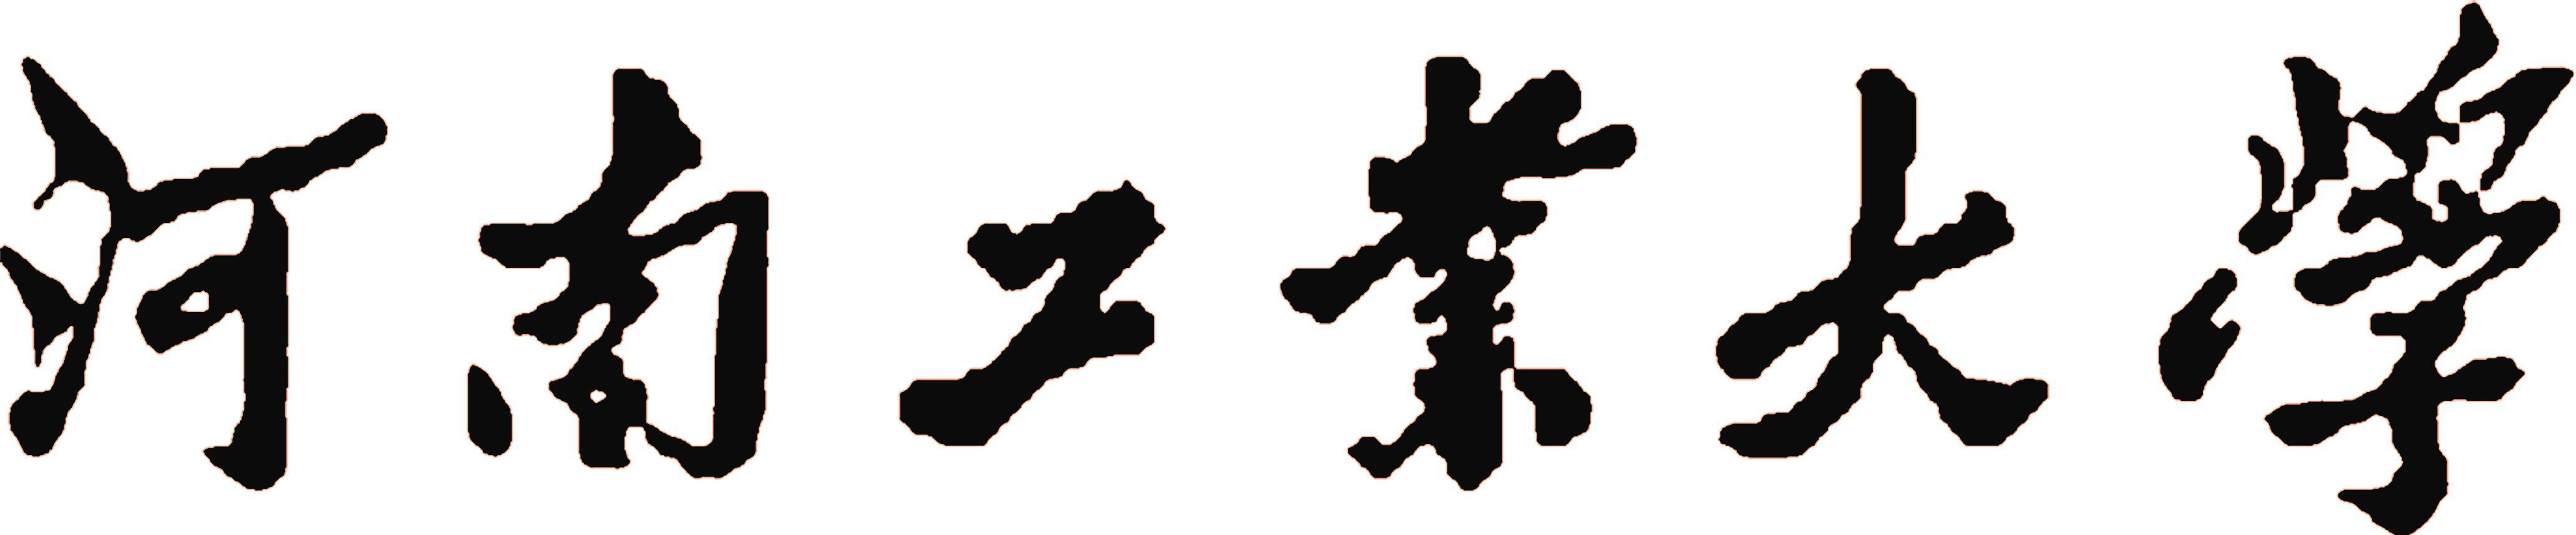
\includegraphics[height=1.6cm]{image/haut_w.png}

\vspace*{3cm}
{\bfseries\zihao{2}{形势与政策课程论文}}

\vfill
{\large
\newcommand{\ctline}[2]{\makebox[4em][s]{\bf #1}:\underline{\makebox[18em][c]{\qquad #2\qquad}}\\[0.4em]}
\ctline{论文题目}{\titlec}
\ctline{专业班级}{软件 1305 班}
\ctline{姓名}{\tjf}
\ctline{学号}{201316920311}
\ctline{辅导老师}{王立璋}
\ctline{完成日期}{\today}
}

\end{center}

\vspace*{2cm}

\end{titlepage}


\title{\titlec}
\author{\tjf\quad 河南工业大学}
\maketitle

\begin{abstract}
中国经济减速已经是有目共睹的事实,而造成这一现象的原因:刘
易斯转折点的迎来和人口红利的消失,都可以归结为计划生育导致的严重少子化。
中国严重少子化对经济发展的不良影响表现在,一个是青年劳动力减少,经济发展将面临
人力资源不足;一个是老龄化加剧,社会负担加重,经济
发展受阻;一个是家庭规模缩小,造成消费需求不足;以及城乡一体化进程的滞缓等。
少子化的出现将给国家经济的可持续发展带来重大威胁和隐患,而国家为促进经济长远发展,
保证经济可持续发展,应当适时地对我国生育政策做出调整,并对养老问题实行更好的政策。

{\bf 关键词:}中国经济减速; 计划生育; 少子化; 人口老龄化
\end{abstract}

\begin{multicols}{2}

在过去 30 年时间里,中国的经济增长速度是一
个奇迹。
目前我国已经超越日本,成为世界上第二大经济
体。中国是由计划经济向市场经济过渡的转轨型国家,
过去的高速经济增长是有目共睹的。

然而近来,数据显示,中国经济减速趋势变得更加鲜明。身边发生的种种,诸如物价变化、用工荒和找工作难、娱乐业繁荣,也无不照应了经济减速的事实。与金融危机时的经济减速比起来,本轮经济减速最大的不同是中国持续高增长的条件、中长期结构性因素,特别是全球化基本面、要素基本面等正在发生趋势性变化。中国经济面临全球金融危机以来最为严重的下滑压力。

\section{中国经济减速原因的归结}

造成中国经济减速的原因有两个。一是中国迎来了刘
易斯转折点。如果发展到某一阶
段,用不变工资招不到工,要想招工必须提高工资时,
刘易斯转折点就来临了 。2004~年是中
国的刘易斯转折点。

第二个因素是中国人口红利的消
失。2010 年进行了第六次人口普察 \cite{jk},这次普察的结
果是劳动型人口绝对减少。扶养比开始上升,
成为人口的转折点。就此,中
国的人口红利消失了 。这对我们的经济增长能力产生
了影响。劳动型人口数绝对减少,劳动力
的增长率显然是负的。投资下降,劳动力负增长,
假设生产率的变化与过去保持一个趋势,那么,潜
在增长率一定会下降。

实质上,这两个原因归结为一点,就是劳动力人口的减少。而劳动力人口的减少,则是由于人口老龄化造成的。在人口基数一定的情况下,老龄人口占据了更大的比例,显然会导致劳动力人口比例的下降。而人口老龄化的根本原因,在于上一代的人口增长率的减缓。人口增长率的减缓有很多原因,对于中国来说则是计划生育的基本国策所导致的。计划生育本身是一项正在调整的政策,所以我们只就其导致的现状来进行分析。与之相似地,我们可以对比日本的少子化现象,来解释中国经济的减速现象。而虽然两国少子化原因大不相同,但所导致的后果是非常相似的。

\section{中国严重少子化的现状和原因}

少子化从宏观上讲可以指一个社会少年儿童
绝对数的减少,也可以理解为少儿人口相对数,即少儿人口总人口比
例下降;从总和生育率的角度理解,少子化指生育率低于人口更
替水平。
就目前我国少子化现象,呈现出三个明显的特征:一是未富
先老,未富先少。
二是城乡少子化程度差距不明显。
三是结构失衡。而这种中国严重少子化的原因,在于以下两点。

{\bf 1. 计划生育政策的实施}

在20世纪50到60年代,我国人口总量迅速增
加,人口规模急剧膨胀。为抑制人口过快增长,缓解巨大的人口压
力,1970年国家出台了“晚婚、晚育、少生、优生”的计划生育政
策,政策规定一对夫妻只生育一个孩子。在计划生育政策实施的30年
左右的时间,我国生育率就呈现出持续下降的趋势。到2010年,
我国提前进入了低生育水平国家行列,且少子化现象
在我国已十分显著与严重。

{\bf 2. 生育观念的改变}

由于我国在短时间内的急速工业化和现代
化,我国儒家传统的传
宗接代思想在西方文化的冲击下,渐渐被国民抛弃。而我国日渐增高
的孩子教育与抚养费用,使得抚养孩子成了家庭的负担。同时随着我
国教育环境的改善和教育水平的提高,各大高校不断扩招,我国高等
教育已步入大众化阶段,高级知识分子愈来愈多。
这些拥有高学历的年轻人崇尚自由、渴求舒适自在的
生活,因此不愿生育孩子给自己带来经济和生活负担。

\section{中国严重少子化对经济发展的不良影响}

虽然目前我国依旧是世界人口第一的国家,人口总额超过13亿
之多。但我们不得不看到,现今我国已处于少子化严重阶段,总
和生育率极为低下。我国在还没实现经济发达、国民富裕时,却呈现出严重
的少子化现象,这将给我国经济的可持续发展造成严重的不良影响。

{\bf 1. 青年劳动力减少,经济发展将面临人力资源不足}

中国人口出生率的迅速下降,带来了时下每年新增劳动力人口
增量的递减,我国
出生率的迅速下降,促成的严重少子化将造成青年劳动力减少,
最终导致我国经济的可持续发展渐渐缺乏新鲜的、有活力的青年劳动
力,国家可利用的人力资源渐少。

{\bf 2. 老龄化加剧,社会负担加重,经济发展受阻}

人口老龄化是指人口结构的变化,是少年儿童人口在总人口中比
重的下降和和老年人口在总人口比重的上升。
在死亡率稳定的情况下,少子化会造成人口金字塔的收缩,底层
幼年人口减少,相对的顶层老年人口则会增加,老龄化程度会进一
步加深。
幼年人口减少,老年人口增
加,这意味着众多老年人都将无子陪伴、生活孤独。这些孤独老人需
要国家、社会给予特别的、贴心的照顾,
这些将耗费和分散国家、社会众多精力与资金,给社会造成
重大压力,抑制经济的发展。

{\bf 3. 家庭规模缩小,造成消费需求不足}

少子化意味着生育率下降,生育率下降的微观人口学后果则
是家庭规模的缩小。
在既定的收入水平下,
每个家庭户人口数减少将带来家庭对生活、文化教育等消费品消费需
求的减少。
我国
家庭规模的缩小导致国内消费需求减少,国民的需求将不能满足我国
日益增多的产品供给,企业生产的产品将面临供过于求的局面,
不利于国家经济健康长远发展。

\section{结语}

中国经济减速已经是有目共睹的事实,而造成这一现象的原因:刘
易斯转折点的迎来和人口红利的消失,都可以归结为计划生育导致的严重少子化。
中国严重少子化对经济发展的不良影响表现在,一个是青年劳动力减少,经济发展将面临
人力资源不足;一个是老龄化加剧,社会负担加重,经济
发展受阻;一个是家庭规模缩小,造成消费需求不足;以及城乡一体化进程的滞缓等。
少子化的出现将给国家经济的可持续发展带来重大威胁和隐患,而国家为促进经济长远发展,
保证经济可持续发展,应当适时地对我国生育政策做出调整,并对养老问题实行更好的政策。
同时在一定程度上,减缓经济发展的步伐,让人口社会发展适合于经济发展,防止出现社会动荡。

\begin{thebibliography}{10}
\bibitem{ren} 从人口学视角论中国经济减速问题. 蔡昉. 中国市场 总第722期.
\bibitem{xw} 怎样看中国人口的现实和未来?. 薛涌. 金融时报中文网, \url{http://www.ftchinese.com/story/001046074}, 2012.
\bibitem{shou} 日本人口少子化问题研究. 施锦芳. 日本研究, 2012(1).
\bibitem{sho} 中日少子化现状及成因分析. 鲁雯霏, 王翾, 汝利娜. 语文学刊, 2014(2).
\bibitem{jj} 中国严重少子化对经济发展的不良影响分析. 廖志琴. 现代经济信息, 2013(11).
\bibitem{jk} 2010年第六次全国人口普查数据公报. 中华人民共和国国家统计局. \url{http://www.stats.gov.cn/tjsj/tjgb/rkpcgb/qgrkpcgb/201104/t20110428_30327.html}, 2011.
\end{thebibliography}

\end{multicols}

\end{document}
